\documentclass[10pt]{beamer}
\usepackage[utf8]{inputenc}
\usepackage{subcaption}
\usepackage{soul}
\usepackage{tikz}
\usetikzlibrary{shapes}

\usepackage{pgfplots}
\usetheme[secheader]{Boadilla}

\usefonttheme[onlylarge]{structurebold}
\setbeamerfont*{frametitle}{size=\normalsize,series=\bfseries}
\setbeamertemplate{navigation symbols}{}

\tikzstyle{noeud}=[minimum width=2.5cm,minimum height=1.5cm,
rectangle,rounded corners=10pt,draw,
fill=blue!5,text=black,font=\footnotesize,text width=2cm,text justified]
\tikzstyle{noeud1}=[minimum width=2.5cm,minimum height=1.1cm,
rectangle,rounded corners=10pt,draw,
fill=green!5,text=black,font=\small,text width=2cm,text centered]
\tikzstyle{varType}=[minimum width=1.5cm,minimum height=0.75cm,
rectangle,rounded corners=10pt,draw,
fill=green!15,text=black,font=\small,text width=2cm,text centered]

\tikzstyle{fleche}=[->,>= stealth,thick]

\title{Statistique Graphique}
\subtitle{EEIA 2024}
\author{Par ...} 
\institute[1]{
      \begin{minipage}{0.1\textwidth}
       
\includegraphics[width=1.6\textwidth, height=1.6\textwidth]{{../../figures/logoFV.jpg}}
       \end{minipage}
       \hspace{0.1\textwidth}
             \begin{minipage}{0.1\textwidth}
             \includegraphics[width=1.6\textwidth, height=1.6\textwidth]{{../../figures/logoBE.png}}
       \end{minipage}
       \hspace{0.1\textwidth}
      \begin{minipage}{0.1\textwidth}
       
\includegraphics[width=1.6\textwidth, height=1.6\textwidth]{{../../figures/Fondation_de_France.png}}
\end{minipage}
}

\date[Godomey 2024]{ \\  Godomey, le 29 juillet 2024 }



\begin{document}
\maketitle

%%%%%%%%%%%%%%%%%%%%%%%%%%%%%%%%%%%%%%%%%%%%%%%%%%%%%%
\begin{frame}
\frametitle {Statistique Graphique}

\begin{columns}
    \begin{column}{0.48\textwidth}
        \begin{block}{Définition}
\small {\begin{itemize}
\item \textbf{Un graphique statistique} : figure fondée sur des données recueillies dans des populations ou des échantillons – Représentation visuelle des variables d’une population
\item Variation \textbf{nouvelle ou inattendue} mise en lumière par la représentation en partant de données complexes
\end{itemize}}
\end{block}
    \end{column}
    \begin{column}{0.48\textwidth}
    \begin{center}
      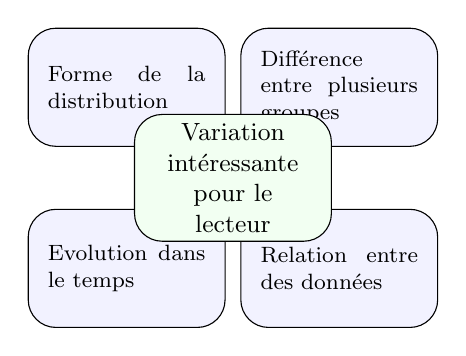
\begin{tikzpicture}  
      \node[noeud] (F) at (0,2.3) { Forme de la distribution};
      \node[noeud] (E) at (0,0) { Evolution dans le temps};
      \node[noeud] (R) at (2.7,0) { Relation entre des données};
      \node[noeud] (D) at (2.7,2.3) { Différence entre plusieurs groupes};
      \node[noeud1] (D) at (1.35,1.15) { Variation intéressante pour le lecteur};
	
        \end{tikzpicture}
      \end{center}
    \end{column}
\end{columns} 

\begin{block}{Objectifs}
\small {\begin{itemize}
\item \textbf{Synthétiser} : En présence de nombreuses données, le cerveau humain a beaucoup de mal à en dégager la configuration. En revanche, avec une représentation visuelle, tout s'éclaire en une seconde !
\item \textbf{Dimension visuelle} : Mémorisation plus simple des faits illustrés car 60 \% de visuels parmi les humains et parce que les faits présentés sont sélectionnés
\item \st{Accompagne un ou des tableau}
\end{itemize}}
\end{block}
\end{frame}
%%%%%%%%%%%%%%%%%%%%%%%%%%%%%%%%%%%%%%%%%%%%%%%%%%%%%%
\begin{frame}
\frametitle {Base de données}
\begin{block}{Définition}
\small {\begin{itemize}
\item Population
\item Attribut/Variable
\end{itemize}}
\end{block}
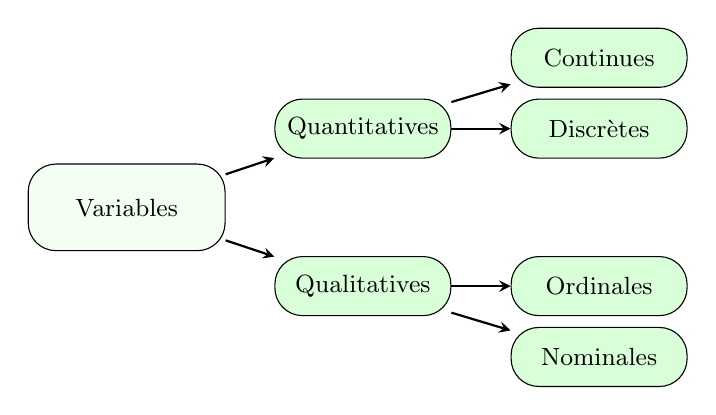
\begin{tikzpicture}
\node[noeud1] (F) at (0,0) {Variables};
\node[varType] (Q) at (3,1) {Quantitatives};
\node[varType] (QC) at (6,1.9) {Continues};
\node[varType] (QD) at (6,1) {Discrètes};

\node[varType] (L) at (3,-1) {Qualitatives};
\node[varType] (LO) at (6,-1) {Ordinales};
\node[varType] (LN) at (6,-1.9) {Nominales};
\draw[fleche] (F)--(Q);
\draw[fleche] (F)--(L);
\draw[fleche] (Q)--(QC);
\draw[fleche] (Q)--(QD);
\draw[fleche] (L)--(LO);
\draw[fleche] (L)--(LN);
\end{tikzpicture}
\end{frame}

\begin{frame}
\frametitle {Base de données: Exemple de Variables}
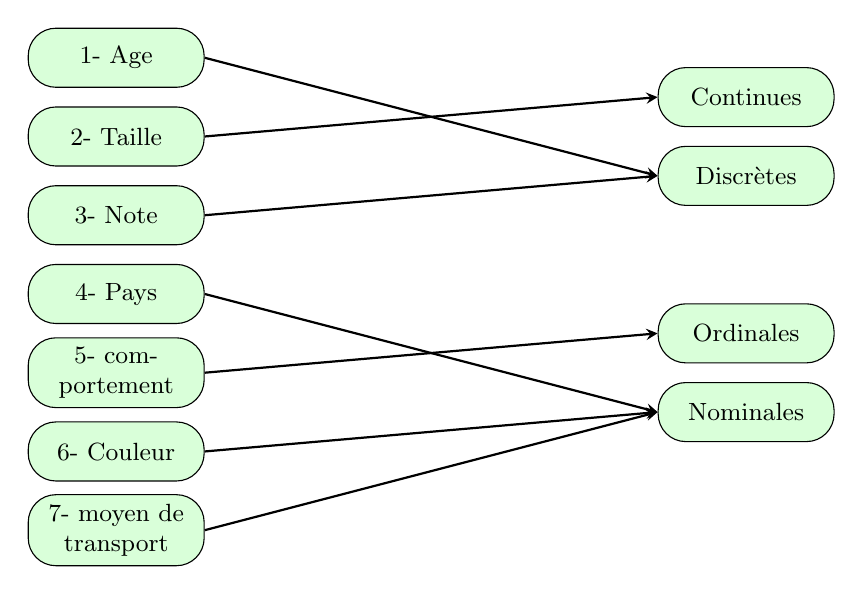
\begin{tikzpicture}
\foreach \nom/\code/\n in {Age/a/1,Taille/b/2,Note/c/3,Pays/d/4,Couleur/f/6,{moyen de transport}/g/7,comportement/e/5}
{\node[varType] (\code) at (0,-\n*1+3.5) {\n - \nom};}
\node[varType] (QC) at (8,2) {Continues};
\node[varType] (QD) at (8,1) {Discrètes};
\node[varType] (LO) at (8,-1) {Ordinales};
\node[varType] (LN) at (8,-2) {Nominales};\pause
\draw[fleche] (a.east)--(QD.west);
\draw[fleche] (b.east)--(QC.west);
\draw[fleche] (c.east)--(QD.west);
\draw[fleche] (d.east)--(LN.west);
\draw[fleche] (f.east)--(LN.west);
\draw[fleche] (g.east)--(LN.west);
\draw[fleche] (e.east)--(LO.west);
\end{tikzpicture}
\end{frame}

\begin{frame}
\frametitle {Statistiques pour synthétiser}
\begin{block}{Localisation}
\small {\begin{itemize}
\item \textbf{Moyenne}
\item \textbf{Médiane}
\item \textbf{Mode et Fréquence}
\end{itemize}}
\end{block}

\begin{block}{Dispersion}
\small {\begin{itemize}
\item \textbf{Ecart type}
\item \textbf{Intervalle interquartile}
\end{itemize}}
\end{block}
\end{frame}

\begin{frame}
\frametitle {Graphes pour synthétiser}
\begin{block}{Distribution}
Pour comprendre la répartition de la variable, ils présentent toutes les valeurs qu'on observe:
\begin{itemize}
\item \textbf{Histogramme} pour les variables quantitatives;
\item \textbf{Barplot} pour les variables qualitatives.
\end{itemize}
\end{block}

\pgfplotstableread[row sep=\\,col sep=&]{
    Notes  & Effectif\\
    8--9   & 2  \\
    10--11 & 11 \\
    12--13 & 8 \\
    14--15 & 7 \\
    16--17 & 2 \\
    18--19 & 1 \\
    }\mydata

\begin{figure}
%\resizebox{!}{5cm}{
\begin{tikzpicture}
    \begin{axis}[
            ybar,
            bar width=20pt,
            symbolic x coords={8--9,10--11,12--13,14--15,16--17,18--19},
            xtick=data,
            height=5cm,
            ytick={1,3,...,12},
            width = 10cm,
            xlabel = Notes,
            ylabel = Effectif
        ]
        \addplot table[x=Notes,y=Effectif]{\mydata};
    \end{axis}
\end{tikzpicture}
%}
\end{figure}
\end{frame}


\begin{frame}
\frametitle {Graphes pour synthétiser}
\begin{block}{Comparaison}
Ils présentent les valeurs observées d'une variable dans différentes catégories:
\begin{itemize}
\item \textbf{Graphique linéaire}  pour les variables quantitatives;
\item \textbf{Barplot} avec plusieurs groupes.
\end{itemize}
\end{block}

\begin{columns}
    \begin{column}{0.48\textwidth}
    \resizebox{\textwidth}{!}{
    %\pgfplotsset{width=7cm,compat=1.18}
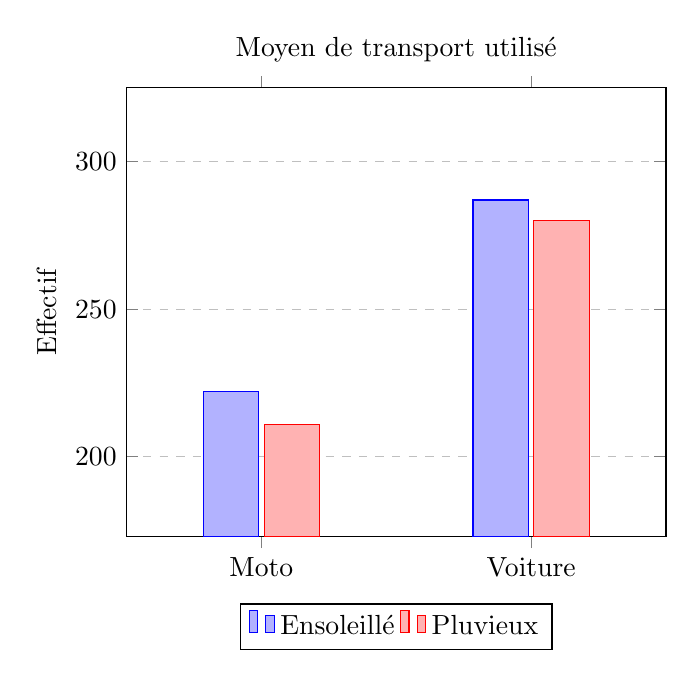
\begin{tikzpicture}
\begin{axis}[ybar,
	title={Moyen de transport utilisé},
    ylabel=Effectif,
    ymajorgrids=true,
    grid style=dashed,,
    enlargelimits=0.5,
    legend style={at={(0.5,-0.15)},
    anchor=north,legend columns=-1},
    bar width=20pt,
    %ybar interval=0.7,
    symbolic x coords={Moto, Voiture},
    xtick=data
]
    \addplot coordinates {
        (Moto,222) (Voiture,287)
    };
    \addplot coordinates {
        (Moto,211) (Voiture,280)
    };
    \legend{Ensoleillé,Pluvieux}
\end{axis}
\end{tikzpicture}
}
    \end{column}
    \begin{column}{0.48\textwidth}
    \begin{figure}
    \pgfkeys{/pgf/number format/.cd,1000 sep={\,}}
\resizebox{\textwidth}{!}{
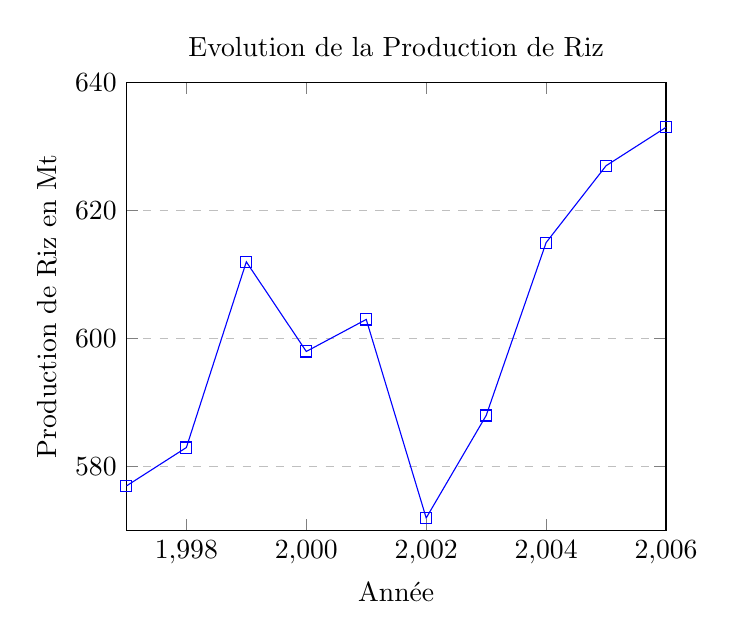
\begin{tikzpicture}
    \begin{axis}[
    title={Evolution de la Production de Riz},
    xmin=1997, xmax=2006,
    ymin=570, ymax=640,
    ymajorgrids=true,
    grid style=dashed,
    xlabel = Année,
    ylabel = {Production de Riz en Mt}
    ]
    \addplot+[sharp plot,
    color=blue,
    mark=square,
    ] coordinates {
        (1997,577) (1998,583) (1999,612)
        (2000,598) (2001,603) (2002,572)
        (2003,588) (2004,615) (2005,627)
        (2006,633)
    };
    \end{axis}
\end{tikzpicture}
}
\end{figure}
    \end{column}
 \end{columns}
\end{frame}


\begin{frame}
\frametitle {Graphes pour synthétiser}
\begin{block}{Relation}
On les utilise quand on cherche à l'impact d'une variable sur une autre:
\begin{itemize}
\item \textbf{Nuage de points} pour deux variables quantitatives;\\
\item \textbf{Boîte à moustache} pour une variable qualitative et une variable quantitative.
\end{itemize}
\end{block}

\end{frame}
\end{document}
